\documentclass{article}
\usepackage{amsmath,amssymb,amsthm,mdframed,kotex,paralist}
\usepackage{tabto}
%\TabPositions{0.5\textwidth}
\TabPositions{0.33\textwidth,0.66\textwidth}
\newcommand\bp[1]{\begin{mdframed}[frametitle={#1},skipabove=10pt,skipbelow=20pt,innertopmargin=5pt,innerbottommargin=40pt]}
\newcommand\ep{\end{mdframed}\par}
\newcommand\ov[1]{\ensuremath{\overline{#1}}}
\newcommand{\vs}{\vspace{0.05\textheight}}
\newcommand{\vvs}{\vspace{0.1\textheight}}
\newcommand{\vvvs}{\vspace{0.15\textheight}}

\begin{document}
\title{석민00 : 수1, 수2, 미적1, 확통 문제들}
\author{}
\date{\today}
\maketitle


\section{수학 1}

\bp{01}
다음을 전개하여라.\par
(1) \((x-1)^3\)\par
(2) \((x+y+2)^2\)
\vs\ep

\bp{02}
다음 방정식과 부등식을 풀어라.\par
(1) \(x^2-18x+45=0\)\par
(2) \(x^3-3x+2=0\)\par
(3) \(2x^2-9x+4<0\)\par
(4) \(|x+1|<5\)
\vvs\ep

\bp{03}
이차방정식 \(x^2+px+q=0\)의 두 근을 \(\alpha\), \(\beta\)라고 할 때, \(|\alpha-\beta|=2\), \(\alpha^2+\beta^2=34\)을 만족시키는 상수 \(p\), \(q\)에 대하여 \(p^2+q^2\)의 값을 구하면?
\vvs\ep

%\bp{04}
%\(x\)에 관한 이차방정식 \(x^2-2(a+k)x+k^2-4k+2b=0\)이 실수 \(k\)의 값에 관계없이 항상 중근을 가질 때, 살수 \(a\)와 \(b\)의 합을 구하면?
%\vvs\ep

\bp{04}
다음 함수의 그래프를 그리시오.\par
(1) \(y=|x^2-2x-3|\).\par
(2) \(x^2-4x+y^2=0\).\par
\vvs
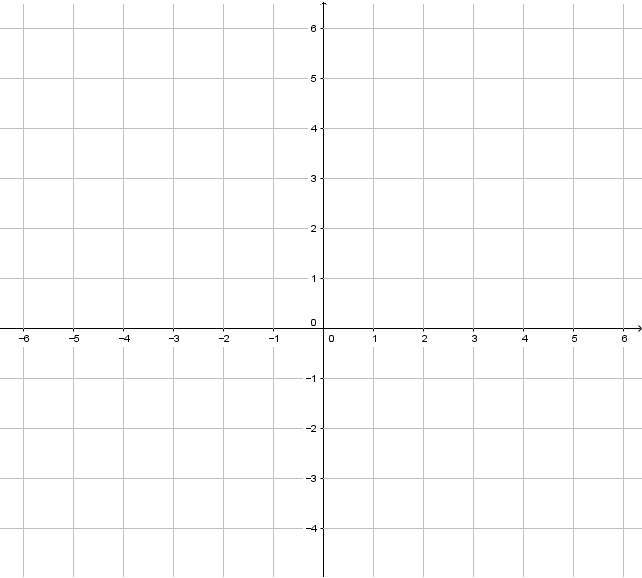
\includegraphics[width=0.45\textwidth]{grid}
~
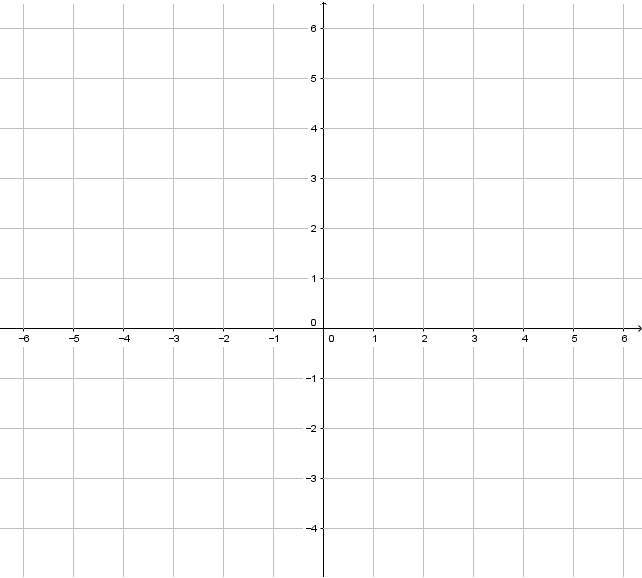
\includegraphics[width=0.45\textwidth]{grid}
\ep

\newpage
\section{수학 2}

\bp{05}
%무리함수 \(y=\sqrt{4-2x}\)의 그래프와 직선 \(y=-x+k\)가 서로 접할 때, \(k\)의 값을 구하시오.
다음 명제의 참 거짓을 판별하시오.\par
(1) \(xy=0\)이면 \(x=0\) 또는 \(y=0\)이다.\par
(2) \(x+y=5\)이면 \(x=2\)이고 \(y=3\)이다.\par
(3) 정수 \(m\)에 대해, \(m\)이 3의 배수이면 \(m^2\)도 3의 배수이다.
\vs\ep

\bp{06}
두 함수 \(f(x)=3x-1\), \(g(x)=-2x+4\)에 대하여 \((g\circ f)^{-1}(2)\)의 값을 구하여라.
\vs\ep

\bp{07}
다음과 같은 수열 \(\{a_n\}\)에서 \(\displaystyle S_5=\sum_{n=1}^5{a_n}\)의 값을 구하시오\par
(1) \(a_n=3n+1\)\par
(2) \(a_n=n^2+n\)\par
(3) \(a_n=2^n\)
\vvs\ep

\bp{08}
(1) \(a>0\), \(b>0\)일 때, \(\frac ab+\frac ba\)의 최솟값을 구하여라.\par\noindent
(2) \(x+y=4\)일 때, \(x^2+y^2\)의 최솟값을 구하여라.
\vs\ep

\section{미분과 적분 1}

\bp{10}
다음을 구하시오.\par
%다음 수열 \(\{a_n\}\)들 중 \(\displaystyle\sum_{n=1}^\infty{a_n}\)가 수렴하는 것을 골라 계산하시오.\par
%(1) \(\displaystyle\lim_{n\to\infty}\frac{4^n}{5^n+3^n}\)\par
%(2) 
(1) \(1+\frac23+\frac49+\frac8{27}+\cdots\)\par
%(3) \(1+\frac1{1+x^2}+\frac1{(1+x^2)^2}+\frac1{(1+x^2)^3}+\frac1{(1+x^2)^4}+\cdots\) (\(x\neq0\))
%(1) \(a_n=4\times\left(\frac12\right)^n\)\par
%(2) \(a_n=3\times(-1)^n\)\par
%(3) \(a_n=\left(\frac1{1+x^2}\right)^{n-1}\)\par
%(4) 
%\vvs\ep

%\bp{11}
%반지름의 길이가 \(1\)인 원에 내접하는 정삼각형을 \(A_1\)이라고 하고, \(A_1\)의 내접원에 내접하는 정삼각형을 \(A_2\)라고 하자.
%이와 같이 정삼각형 \(A_n\)의 내접원에 내접하는 정삼각형을 \(A_{n+1}\)(\(n=1,2,3,\cdots\)), \(A_n\)의 넓이를 \(a_n\)이라고 할 때, \(\displaystyle\sum_{n=1}^{\infty}a_n\)의 값을 구하여라.
%\vvs\ep
%
%\bp{11}
%다음을 구하시오.\par
(2) \(\displaystyle\lim_{x\to\infty}\frac{5x^2-4x+1}{2x^2+3x-5}\)\par
(3) \(\displaystyle\lim_{x\to0}\frac{\sqrt{2+x}-\sqrt2}{\sqrt2x}\)\par
\vs\ep

\bp{11}
다음을 만족하는 상수 \(a\), \(b\)의 값을 구하시오.
\[
\lim_{x\to2}\frac{x^2+ax+b}{x-2}=5
\]
\vs\ep

\bp{12}
다음 \(0\le x\le 3\)일 때 \(y\)의 최솟값을 구하시오.\par
(1) \(y=x^3-3x+6\).\par
(2) \(y=x^4-6x^2-8x+10\)
\vs\ep

\bp{13}
다음을 구하시오.\par
(1) \(\int_0^3|x-1|\,dx\)\par
(2) \(\int_0^3x^2-2x+2\,dx\)
\vs\ep

%\bp{13}
%(1)
%\(y=x^2\)에 접하고 \((-1,-3)\)을 지나는 두 접선을 구하시오.\\
%(2)
%(1)에서 구한 두 접선과, 원래의 곡선이 만드는 영역의 넓이를 구하시오.
%\vvvs\ep

%\bp{18}
%정적분을 이용하여 다음 극한값을 구하여라.
%\[
%\lim_{n\to\infty}\sum_{k=1}^n\left(1+\frac2nk\right)^3\cdot\frac1n
%\]
%\vvs\ep

%\bp{19}
%(1) \(f(x)=(2x+1)^4\)일 때, \(f'(-1)\)을 구하시오.
%
%\noindent
%(2) \(f(x)=x^3-6x^2+5\)이고 \(0\le x\le 6\)일 때 \(f(x)\)의 최댓값을 구하시오.
%\vvs\ep

\section{확률과 통계}

\bp{14}
다음과 같은 그림에서 \(A\)에서 \(B\)로 최단거리로 가는 경로의 개수를 구하시오.
{\center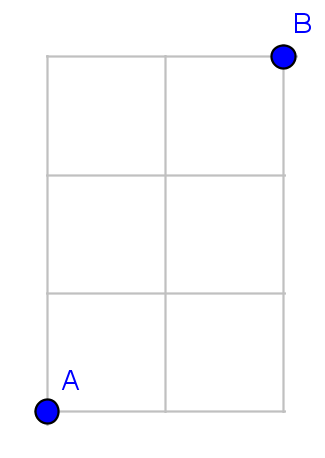
\includegraphics[width=0.2\textwidth]{path}}
\vs\ep

\bp{15}
success의 7개의 문자를 모두 일렬로 나열할 때 다음 물음에 답하여라\par
(1) 나열할 수 있는 모든 경우의 수를 구하시오.\par
(2) 세 개의 s가 모두 이웃하도록 나열되는 경우의 수를 구하시오.\par
(3) 7개의 문자를 임의로 나열할 때, 세 개의 \(s\)가 모두 이웃하도록 나열될 확률을 구하시오.
\vvs\ep

\bp{16}
\((x+1)^7=a_7x^7+a_6x^6+\cdots+a_1x+a_0\)
일 때, \(a_4\)의 값을 구하시오.
\vvs\ep

\bp{17}
다음을 구하여라\par
(1) \(P(5,3)\)\par
(2) \(S(5,3)\)
\vvs\ep

\bp{18}
주사위를 180번 던질 때 1의 눈이 나오는 횟수를 \(X\)라고 하자.\par
(1) \(E(X)+V(X)\)를 구하시오.\par
(2) \(Y=2X+1\)일 때, \(E(Y)+V(Y)\)를 구하시오.
\vvs\ep
\end{document}